\documentclass[17pt]{beamer}
\usepackage{geometry}
\geometry{papersize={21cm,15.75cm}}

\beamertemplatenavigationsymbolsempty

%%%% CANVAS %%%%%
\setbeamertemplate{background canvas}[vertical shading][bottom=black!80!blue!90,top=black!100]

%%%% OUTER %%%%%
\useoutertheme{infolines}
\setbeamercolor{section in head/foot}{fg=yellow, bg=black!70!blue!90}
\setbeamerfont{section in head/foot}{size=\fontsize{12}{12}\selectfont\vspace*{-2pt}}

\setbeamercolor{subsection in head/foot}{fg=white, bg=black!70!blue!90}
\setbeamerfont{subsection in head/foot}{size=\fontsize{12}{12}\selectfont\vspace*{-2pt}}

\setbeamercolor{title in head/foot}{fg=white, bg=}
\setbeamerfont{title in head/foot}{size=\fontsize{12}{12}\selectfont\vspace*{1pt}}
\setbeamercolor{date in head/foot}{fg=white, bg=}
\setbeamerfont{date in head/foot}{size=\fontsize{12}{12}\selectfont\vspace*{-1pt}}
\setbeamercolor{author in head/foot}{fg=white, bg=}
\setbeamerfont{author in head/foot}{size=\fontsize{12}{12}\selectfont\vspace*{2pt}}

%%%%% BLOCKS + INNER %%%%%

\useinnertheme{default}
\setbeamercolor{block body}{bg=, fg=white}
\setbeamercolor{block title}{bg=, fg=white}
\setbeamerfont{block title}{series=\bfseries, size=\normalsize}

\setbeamercolor{alerted text}{fg=red}
\setbeamercolor{block body alerted}{bg=, fg=white}
\setbeamercolor{block title alerted}{bg=,fg=red}

\setbeamercolor{block body example}{bg=, fg=white}
\setbeamercolor{block title example}{bg=, fg=green}

\setbeamercolor{fine separation line}{}
\setbeamercolor{frametitle}{fg=yellow}
\setbeamercolor{item projected}{fg=white}
\setbeamercolor{normal text}{bg=,fg=white}
\setbeamercolor{structure}{bg=, fg=yellow!70}

\setbeamercolor{title}{fg=white}
\setbeamerfont{title}{size=\huge}
\setbeamercolor{author}{fg=white}
\setbeamerfont{author}{size=\Large}
\setbeamercolor{titlelike}{fg=white}

\newlength{\halfwidth}
\newlength{\halfheight}
\setlength{\halfwidth}{0.5\textwidth}
\setlength{\halfheight}{0.42\textheight}

\newcommand{\blockinclude}[1]
{
  \fontsize{12pt}{12pt}\selectfont
  \setbeamertemplate{blocks}[rounded]{~}
  \setbeamercolor{block body}{bg=white, fg=black} %
  \begin{block}{}\centering\include{#1}\end{block}
}

\newcommand{\blockincludetwo}[2]
{
  \fontsize{12pt}{12pt}\selectfont
  \setbeamertemplate{blocks}[rounded]{~}
  \setbeamercolor{block body}{bg=white, fg=black} %
  \begin{block}{}
    \centering 
    \resizebox{.5\halfwidth}{\halfheight}{
      \begin{minipage}{\halfwidth}
        \include{#1}
      \end{minipage}
    }
    \resizebox{\halfwidth}{!}{
      \begin{minipage}{\halfwidth}
        \include{#2}
      \end{minipage}
    }
  \end{block}
}

%%%%%%%%%%%%%%%%%%%%%%%%%%%%%%%%%%%%%%%%%%%%%%%%%%%%%%%%%%%%%%%%%%%%%%%%%%%%%% 

\usepackage[utf8]{inputenc}
\usepackage{multirow}

% MATH
\usepackage{amssymb}
\usepackage{amsmath}
\usepackage{mathtools}
%\usefonttheme[onlymath]{serif}

% IMAGES
\usepackage{graphicx}
\usepackage{epstopdf}
\makeatletter \def\input@path{{Graphics/}} \makeatother
\graphicspath{{./MCRapport/}{./Graphics/}}
\usepackage{caption}
\usepackage{tikz}
\usetikzlibrary{positioning, calc, shapes, arrows}
% MACRO

\newenvironment{blockitemize}[1]{
  \begin{block}<+->{#1}
    \begin{itemize}
    }{
    \end{itemize}
  \end{block}
}

\newenvironment{blockenumerate}[1]{
  \begin{block}<+->{#1}
    \begin{enumerate}
    }{
    \end{enumerate}
  \end{block}
}

\newcommand{\F}{\mathcal{F}}
\newcommand{\U}{U_{[0,1]}}
\newcommand{\err}{e_{L^2}}
\newcommand{\rb}{\textcolor{red}{\textbullet}}

\title[Modélisation transport]{Modélisation de transport de particules neutres}
\author[Sohet \& Valade]{a.k.a}
\date{}

\begin{document}

\begin{frame}
  \maketitle
  \centering
  \vspace{-40pt}
  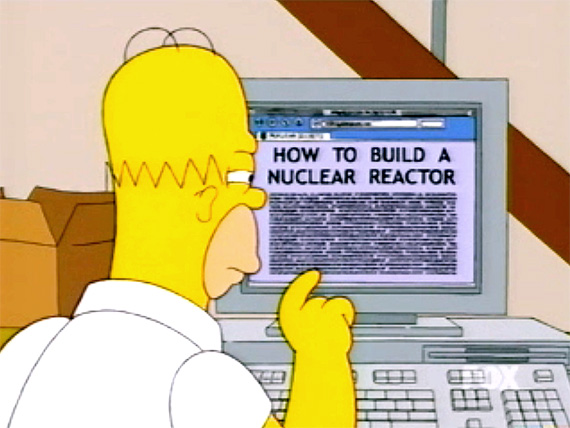
\includegraphics[height=.55\textheight]{homer_simpson_reading_on_pc}
\end{frame}

\section{Introduction}
\begin{frame}{Introduction}
  \begin{blockitemize}{But du TP}
  \item Modélisation de transport de particules neutres
  \item Compréhension des équations de Boltzmann 
  \item Implémentation des cas monodimentionnels 
  \end{blockitemize}

  \begin{blockitemize}{Méthodes employées}
  \item Méthode Monte-Carlo
    \begin{itemize}
    \item Particule par particule
    \item Méthode stochastique
    \end{itemize}
  \item Méthode Déterministe
    \begin{itemize}
    \item Toutes les particules ensemble...
    \item Mais rebond par rebond ou pas par pas
    \end{itemize}
  \end{blockitemize}
\end{frame}

\begin{frame}{Études menées}
  \begin{block}<+->{Équation de Bolztmann 1D}
    \[
      \underbrace{\mu \partial_x \phi(\mu, x) + \Sigma_t \phi(\mu, x)}_{\text{Libre parcours en milieu asborbant}}
      =
      \underbrace{S(x)}_{\text{Source}} + \underbrace{\frac{\Sigma_s}{2} \int_{-1}^1 \phi(\mu', x) d\mu'}_{\text{Diffusion}}
    \]
  \end{block}
  \begin{blockitemize}{Cas particuliers étudiés}
  \item Type de source
    \begin{itemize}
    \item Ponctuelle en 0
    \item Constante sur le segment $[0,1]$
    \end{itemize}
  \item Type d'absorbtion
    \begin{itemize}
    \item Constante sur le segment $[0,1]$
    \item Avec une marche de facteur $3$ entre $0.3$ et $0.7$
    \end{itemize}
  \item Type de diffusion
    \begin{itemize}
    \item Avec
    \item Sans
    \end{itemize}
  \end{blockitemize}
\end{frame}

\section{Problèmes sans diffusion}

\begin{frame}
  \tableofcontents[currentsection]
\end{frame}

\subsection{Propagateur et Monte-Carlo}

\begin{frame}{Idée générale}
  \begin{blockitemize}{Approche}
  \item On se donne un (grand) nombre de particules...
  \item Et une discrétisation dans l'espace
  \item On fait ``voyager'' les particules une par une
  \item On utilise des variables aléatoires
  \end{blockitemize}

  \begin{blockitemize}{Algorithme sans diffusion}
  \item[\rb] Pour chaque particule
    \setlength\itemindent{35pt}
  \item Générer la particule avec la source adaptée
  \item Lancer la particule avec une probabilité de libre parcours
    \setlength\itemindent{0pt}
  \item[\rb] Fin pour
  \item Calculer la répartition finale des particules
  \end{blockitemize}
\end{frame}

\begin{frame}{Propagateur}
  \begin{blockitemize}{Nécessité}
  \item Coeur du code
  \item Représente la physique du libre parcours 
  \end{blockitemize}
  \begin{blockenumerate}{Création à partir d'une loi uniforme unitaire}
  \item Trouver la loi de probabilité théorique de diffusion en fonction du milieu
  \item Calculer sa fonction de répartition et l'inverser
  \item On a maintenant
    \[ X = \F^{-1}\big(\U\big) \]
    \[ 0\leq X \leq \infty\]
  \end{blockenumerate}
\end{frame}

\begin{frame}{Propagateur}{Propagateurs utilisés}
  \begin{blockitemize}{Absorption constante}
  \item Loi de probabilité du libre parcours physique
    \[ P(X=l) = \frac{\Sigma_t}{\mu} e^{\frac{-\Sigma_t}{\mu}l} \]
  \item Variable aléatoire dérivée 
    \[ X = -\frac{\mu}{\Sigma_t}\log\big(\U\big) \]
  \end{blockitemize}
  \vspace{-10pt}
  \begin{blockitemize}{Absorption avec marche}
  \item Variable aléatoire dérivée de la physique, avec $C_{1, 2, 3}(\lambda), \mu(\lambda)$ 
    \[ X =
      \begin{cases}
        -\mu \log(C_1- \U/\lambda)                                  & \U<0.3\\
        \tfrac{1}{3} \big(0.6 - \mu \log(3(C_2 - \U/\lambda))\big)  & 0.3<\U<0.7\\
        -0.8 - \mu \log(C_3 - \U/\lambda)                           & 0.7<\U
      \end{cases}
    \]
  \end{blockitemize}
\end{frame}


\subsection{Schéma diamant et méthode déterministe}

\begin{frame}{Schéma diamant}
  \begin{blockitemize}{Idée}
  \item Toutes les particules au point $x$ sont considérées
  \item Elles avancent toutes ensemble dans la bonne direction
  \end{blockitemize}
  \begin{blockitemize}{Équation}
  \item Schéma basé sur des ``pseudo'' volumes finis
  \item Pour $\mu>0$
    \[
      \phi_{i+1} = \frac{2 dx_i S(x_i)}{\eta^+} +
      \frac{\eta^-}{\eta^+}\phi_{i}, \qquad \eta^\pm = 2\mu \pm dx_i\Sigma_t(x_i)
    \]
  \item \textcolor{red}{Condition} : Le rapport $\eta^-/\eta^+$ doit être compris entre zéro et un
  \item Même idée pour $\mu<0$ mais on parcourt les $x_i$ de un à zéro
  \end{blockitemize}
\end{frame}


\subsection{Résultats}

\begin{frame}{Résultats pour une absorption constante}{Source ponctuelle}
  \only<1>{
    \begin{figure}
      \centering
      \includegraphics[width=.9\textwidth]{phi_sigma_cst_source_delta}
      \caption{Résultats Monte-Carlo et théorique pour une source en $\delta(0)$ avec $\mu=0.5$ et $\Sigma_t=3$. On a $\err \approx 10^{-6}$.}
    \end{figure}
  }
  \only<2>{
    \begin{figure}
      \centering
      \blockinclude{output_1_05_5_2}
      \caption{Exemple de résultat du solveur ``diamant'' pour un cas sans diffusion, $\mu=-1, \sigma=5$ et un source constante sur $[0,1]$. On a $\err \approx 10^{-3}$ pour $N_x=10^3$.}
      \label{fig:exple_a}
    \end{figure}
  }
\end{frame}
\begin{frame}{Résultats pour une absorption constante}{Source constante}
  \only<1> {
    \begin{figure}
      \centering
      \includegraphics[width=.9\textwidth]{phi_sigma_cst_source_cste}
      \caption{Résultats Monte-Carlo et théorique pour une source constante avec $\mu=0.5$ et $\Sigma_t=3$. On a $\err \approx 10^{-6}$.}
    \end{figure}
  }
  \only<2> {
    \begin{figure}
      \centering
      \blockinclude{output_1_1_5_1}
      \caption{Exemple de résultat du solveur ``diamant'' pour un cas sans diffusion, $\mu=1, \sigma=5$ et un source constante sur $[0,1]$. On a $\err \approx 10^{-3}$ pour $N_x=10^3$.}
      \label{fig:exple_b}
    \end{figure}
  }
\end{frame}

\begin{frame}{Résultats pour une absorption avec une marche}
  \only<1>{
    \begin{figure}
      \centering
      \includegraphics[height=.75\textheight]{TP1_sigmavar}
      \caption{Résultats Monte-Carlo et théorique pour une source en $\delta(0)$ avec $\mu=0.5$ et sigma discontinu. On a $\err \approx 10^{-6}$.}
    \end{figure}
  }
  \only<2> {
    \begin{figure}
      \centering
      \blockinclude{output_two_steps_1_05_1_2}
      \caption{Courbes théorique et expérimentale pour $\sigma_t(x)$ avec une marche. On prend ici $\mu=.5$. On a $\err \approx 10^{-3}$ pour $N_x=10^3$.}
      \label{fig:ts_05}
    \end{figure}
  }
  \only<3> {
    \begin{figure}
      \centering
      \blockinclude{output_two_steps_1_05_3_2}
      \caption{Courbes théorique et expérimentale pour $\sigma_t(x)$ avec une marche. On prend ici $\mu=.5$, mais on prend aussi un coeficient multiplicatif sur $\Sigma_t$ d'un facteur $3$.  On a $\err \approx 10^{-3}$ pour $N_x=10^3$.}
      \label{fig:ts_3}
    \end{figure}
  }
\end{frame}

\section{Problèmes avec diffusion}

\begin{frame}
  \tableofcontents[currentsection]
\end{frame}

\subsection{Monte-Carlo diffusif}

\begin{frame}{Ajout de la diffusion}
  \only<1> {
    \textcolor{red}{On travaille particule par particule}
    \begin{blockitemize}{Modifications majeures}
    \item La particule \textcolor{red}{peut} rebondir après chaque libre parcours ...
    \item Ou sortir du domaine ...
    \item Ou être absorbée
    \item Il faut donc une nouvelle variable aléatoire pour en décider
    \item Il faut aussi noter la position de la particule à chaque rebond
    \end{blockitemize}
  }
  \only<2> {
    \begin{blockitemize}{Nouvel algorithme}
    \item[\rb] Pour chaque particule
      \setlength\itemindent{35pt}
    \item Générer la particule avec la source \textcolor{red}{isotrope} adaptée 
    \item[\rb] Faire
      \setlength\itemindent{70pt}
    \item Noter la position
    \item Calculer une variable aléatoire de probabilité de diffusion
      \begin{itemize}
        \setlength\itemindent{70pt}
      \item Sortir si nécessaire
      \end{itemize}
    \item Tirer une nouvelle direction aléatoire
    \item Lancer la particule avec une probabilité de libre parcours 
      \setlength\itemindent{35pt}
    \item[\rb] Tant que non absorbée et dans le domaine
      \setlength\itemindent{0pt}
    \item[\rb] Fin pour
    \item Calculer la répartition finale des particules avec tous les rebonds
    \end{blockitemize}
  }
\end{frame}

\subsection{Code déterministe}

\begin{frame}{Modifications du code déterministe}
  \only<1> {
    \textcolor{red}{On travaille rebond par rebond}
    \begin{blockitemize}{Modifications majeures} 
    \item Il faut une quadrature pour intégrer sur l'ensemble des directions 
    \item A chaque boucle il faut faire circuler toutes les populations à direction donnée
      \begin{itemize}
      \item Et dans le bon sens...
      \end{itemize}
    \item Chaque ancienne population ayant diffusé sera ajoutée à un terme source modifié et on relance l'expérience... 
    \item Jusqu'à arriver à un profil stable
    \end{blockitemize}
  }
  \only<2> {
    \begin{blockitemize}{Algorithme modifié}
    \item Calculer les points de quadratures pour la diffusion 
    \item Initialiser la source modifiée avec la source classique
    \item[\rb] Faire
      \setlength\itemindent{35pt}
    \item[\rb] Pour toute direction de la quadrature
      \setlength\itemindent{70pt}
    \item Fixer la bonne condition au bon bord 
    \item Faire ``avancer'' le flux dans la bonne direction
    \item Calculer la contribution de la direction au flux total
      \setlength\itemindent{35pt}
    \item[\rb] Fin pour
    \item Calculer la nouvelle source modifiée
      \setlength\itemindent{0pt}
    \item[\rb] Tant que deux sources modifiées consécutives sont trop différentes 
    \end{blockitemize}
  }
\end{frame}

\subsection{Ajout de la DSA}

\begin{frame}{Limite du code déterministe}
  \begin{blockitemize}{Problèmes} 
  \item La boucle continue tant qu'il y a beaucoup de particules en mouvement
  \item Cela peut prendre très longtemps (voire ne pas converger) dans les cas suivant
    \begin{itemize}
    \item Absorption faible
    \item Diffusion forte
    \item Source forte
    \end{itemize}
  \item Les termes de hautes fréquences spaciales sont anéantis...
  \item Mais les termes de diffusion basse fréquence ne le sont pas 
  \end{blockitemize}
\end{frame}

\begin{frame}{Méthode de DSA}
  \begin{blockitemize}{Modification de la méthode classique} 
  \item Résoudre de manière Jusqu'à calculer $Q_{i+1}$, la nouvelle source modifiée.
  \item Résoudre le problème de diffusion pure liée
    \[
      -\frac{1}{3\Sigma_t}\partial_x^2 f + \Sigma_t f = \Sigma_s [Q_{i+1}-Q_i] 
    \]
  \item Ajouter la solution obtenue
    \[
      Q_{i+1} \leftarrow Q_{i+1} + f 
    \]
  \end{blockitemize}

  \begin{blockitemize}{Résolution de l'équation}
  \item Formalisation pour des élements finis en une dimension
  \item Inversion de la matrice avec l'algorithme fourni par Eigen
    \begin{itemize}
    \item Méthode de Cholesky directe dite LLTD
    \end{itemize}
  \end{blockitemize}
\end{frame}


\subsection{Résultats}

\begin{frame}{Source ponctuelle}
  \only<1> {
    \begin{figure}
      \centering
      \includegraphics[height=.7\textheight]{TP1_diff_delta}
      \caption{Courbes expérimentales pour une source constante sur $[0,1]$. Lancer de $2\cdot10^6$ particules avec $\Sigma_a = 1, \Sigma_s = 5$.}
      \label{fig:TP1_diff}
    \end{figure}
    }
\end{frame}

\begin{frame}{Source continue}
  \only<1>{
    \begin{figure}
      \centering
      \includegraphics[height=.7\textheight]{TP1_diff} \\
      \caption{Courbes expérimentales pour une source ponctuelle en 0. Lancer de $2\cdot10^6$ particules avec $\Sigma_a = 1, \Sigma_s = 5$.}
      \label{fig:TP1_diff}
    \end{figure}
  }
\end{frame}

\begin{frame}{Nombre sauts en Monte-Carlo}
  \begin{figure}
    \centering
    \includegraphics[height=.7\textheight]{TP1_diff_nb_jumps}
    \caption{Distribution du nombre de particules en fonction du nombre de sauts pour un lancer de $2\cdot10^6$ particules, avec $\Sigma_a = 1, \Sigma_s = 5$, et un source constante sur $[0,1]$.}
    \label{fig:nbjumps}
  \end{figure}
\end{frame}

\begin{frame}{Vitesse en convergence en déterministe}
  \begin{table}
    \centering
    \begin{tabular}{c|ccc}
      $\varepsilon $ & .1 & 0.01 & 0.001 \\
      \hline
      Boucles \textit{sans} DSA & 761 & $>10^5$ & $>10^5$ \\
      Boucles \textit{avec} DSA & 32 & 46 & 313 \\
      \hline
      Tps calcul \textit{sans} DSA & 2.9 & 40 & 40 \\
      Tps calcul \textit{avec} DSA & 0.15 & 0.22 & 1.5 \\
    \end{tabular}
    \caption{Vitesses de convergence pour les schémas avec ou sans DSA.}
    \label{tab:DSA}
  \end{table}
\end{frame}

\begin{frame}{Erreur en fonction du nombre de particules}
  \begin{figure}
    \centering
    \includegraphics[width=.8\textwidth]{error_n_parts}
    \caption{Erreur entre solution exacte et solution approximée en fonction du nombre de particules.}
    \label{fig:vcv}
  \end{figure}
\end{frame}

\begin{frame}{Erreur en fonction du nombre de segments}
  \only<1>{
    \begin{figure}
      \centering
      \blockinclude{nb_segs_diff_L2_delta}
      \caption{Courbe de la distance relative de l'approximation à la solution exacte en fonction du nombre de pas de la discrétisation spatiale. Le cas présenté ici est celui d'une source ponctuelle en 0.}
      \label{fig:Nx_diff_d}
    \end{figure}
  }
  \only<2> {
    \begin{figure}
      \centering
      \blockinclude{nb_segs_diff_L2_cste}
      \caption{Courbe de la distance relative de l'approximation à la solution exacte en fonction du nombre de pas de la discrétisation spatiale. Le cas présenté ici est celui d'une source constante unitaire sur le segment $[0,1]$.}
      \label{fig:Nx_diff_c}
    \end{figure}
  }
\end{frame}

\begin{frame}{Convergence en fonction de la quadrature}
  \only<1> {
    \begin{figure}
      \centering
      \blockinclude{loop_nb_pts_mu_delta}
      \caption{Courbes pour différents niveaux de discrétisation de $N_\mu$ dans le cas d'une experience à source en $\delta(0)$.}
      \label{fig:lm_d}
    \end{figure}
  }
  \only<2> {
    \begin{figure}
      \centering
      \blockinclude{loop_nb_pts_mu_cste}
      \caption{Courbes pour différents niveaux de discrétisation de $N_\mu$ dans le cas d'une experience à source constante unitaire sur $[0,1]$.}
      \label{fig:lm_c}
    \end{figure}
  }
\end{frame}

\begin{frame}{$\epsilon-$Experience }
      \begin{figure}
      \centering
      \blockinclude{output_limit_sigma_a_zero}
      \caption{Courbes théorique pour le cas limite $\epsilon=0$ et expérimentale pour $\sigma_a=0$ et $\epsilon=0.001$.}
      \label{fig:limit_sigma_zero}
    \end{figure}
\end{frame}


\section{Conclusion}

\begin{frame}{Conclusion}
  \begin{blockitemize}{Points à améliorer}
  \item Études comparatives plus poussées entre déterministe et Monte-Carlo
    \begin{itemize}
    \item Vitesse de convergence
    \item Précision
    \item Adaptabilité
    \end{itemize}
  \item Utilisation du schéma upwind
  \end{blockitemize}
  \begin{blockitemize}{Idées d'aprofondissement}
  \item Utiliser des coefficients non constants plus complexes
  \item Passer en plusieurs dimensions...
  \end{blockitemize}
  \centering
  \uncover<3>{
    \includegraphics[height=.4\textheight]{homer_woohoo}
  }
\end{frame}
\end{document}
%%% Local Variables:
%%% mode: latex
%%% TeX-master: t
%%% End:
